\documentclass[10pt, compress]{beamer}

\usetheme{metropolis}
\usepackage{appendixnumberbeamer}

\usepackage{tikz-dependency}
\usepackage{caption}
\usepackage{booktabs}
\usepackage{tabularx}
\usepackage{alltt}
\usepackage[scale=2]{ccicons}

\usepackage{pgfplots}
\usepgfplotslibrary{dateplot}

\usepackage{xspace}
\newcommand{\themename}{\textbf{\textsc{metropolis}}\xspace}

% commands from the paper
\newfontfamily\gtfont[Scale=1.1,Letters=SmallCaps]{Linux Libertine O}
\newcommand{\udtag}[1]{{\ll \textsc{#1}}}
\newcommand{\gtlabel}[1]{{\gtfont #1}}
\newcommand{\udlabel}[1]{{\tt #1}}
\newfontfamily\udfont[Scale=0.9,Letters=SmallCaps]{Linux Libertine O}
\newcommand{\utag}[1]{{\udfont#1}}
\newcommand{\ufeat}[1]{{\udfont#1}}
\newcommand{\tgl}[1]{{\em #1}}
\setmonofont[Scale=MatchLowercase]{DejaVu Sans Mono}

% commands from the paper


\newcommand{\myarrow}[1][-45]{%
  \mathrel{%
    \text{$
     \begin{tikzpicture}[baseline = -0.5ex]
       \node[inner sep=0pt,outer sep=0pt,rotate = #1] (a) at (0,0)  {$\xrightarrow{}$};
    \end{tikzpicture}
    $}%
  }%
}%




\title{Class 01: Getting started }

\begin{document}

\maketitle

\begin{frame}{Why are you taking this course?}

Either:
\begin{itemize}
  \item You don't know programming but are eager to learn, or
  \item It's a requirement for your degree
\end{itemize}

Good news!
\begin{itemize}
  \item Programming is fun
  \item Programming improves all aspects of human experience
  \item Programming will make your life easier
\end{itemize}

More good news! 
\begin{itemize}
  \item All the examples are based on linguistic problems
\end{itemize}

\end{frame}

\begin{frame}{Prerequisites}

Stuff you need before you begin:
\begin{itemize}
 \item A UNIX-compatible system (GNU/Linux, *BSD, Mac/OS)
 \item A text editor
 \item An installation of Python -- Python 3.0 or higher!
\end{itemize}

How to choose a text editor:

\begin{center}
  
\includegraphics[width=0.6\textwidth]{graphics/realprogrammers.png}
\end{center}

Honestly, use something other people (programmers) you know use.

\end{frame}

\begin{frame}{Argh but what if I have Windows™}

\begin{center}
I have no idea about Windows
\end{center}

To be safe, install a Virtual Machine (e.g. VirtualBox) and a flavour
of GNU/Linux, e.g. Ubuntu.

\end{frame}

\begin{frame}{How to get help}

\begin{center}
  \begin{onlyenv}<1>
  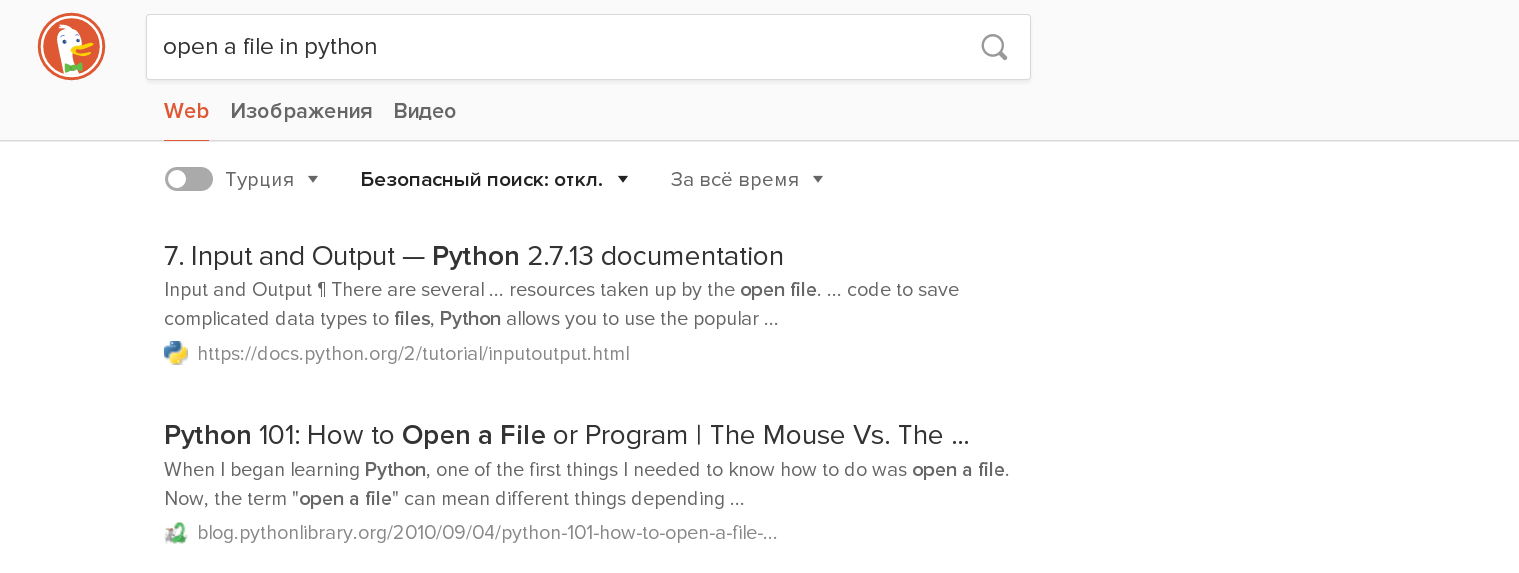
\includegraphics[width=0.6\textwidth]{graphics/duckduckopenfile.png}
  \end{onlyenv}
  \begin{onlyenv}<2>
  
\includegraphics[width=0.6\textwidth]{graphics/pythondocs.png}
  \end{onlyenv}
  \begin{onlyenv}<3>
  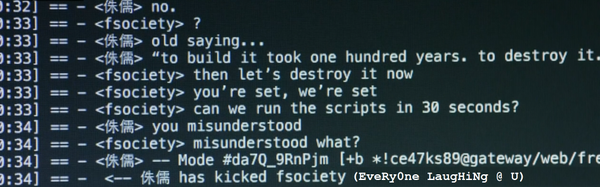
\includegraphics[width=0.6\textwidth]{graphics/CKmO8DXVAAAWl1d.png}
  \end{onlyenv}
  \begin{onlyenv}<4>
  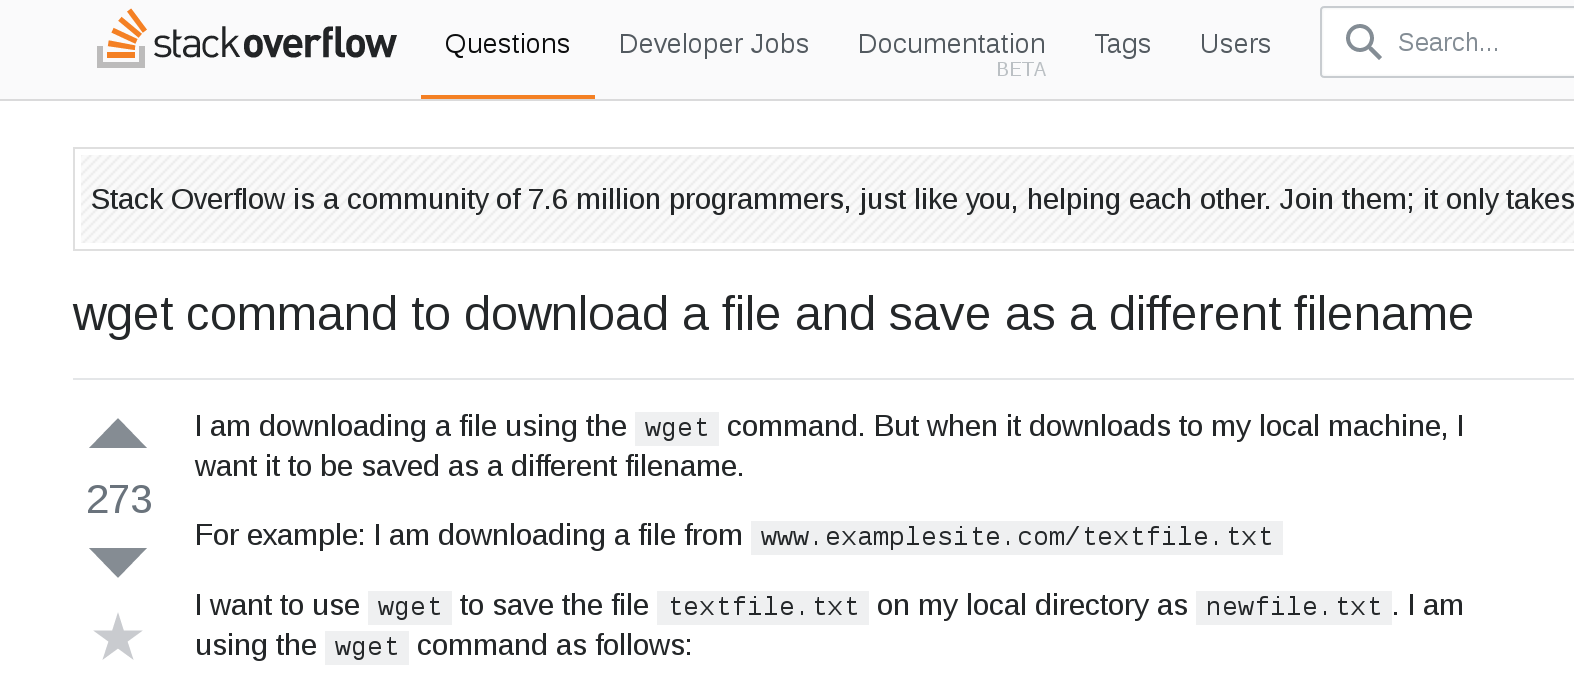
\includegraphics[width=0.6\textwidth]{graphics/stackoverflow.png}
  \end{onlyenv}
\end{center}

\textbf{On your own:}
\begin{itemize}
  \item A search engine such as Google™, Yandex™ or DuckDuckGo™
  \item The fine Python documentation: \url{http://docs.python.org}
  \item Internet Relay Chat: \url{http://webchat.freenode.net}
  \item Stack Overflow: \url{https://stackoverflow.com}
\end{itemize}

\begin{center}
\begin{tabularx}{\textwidth}{lXrl}
   \textbf{Ask me:} &       In class & (IRL) \\
                 & {\tt \#hseling} on {\tt irc.freenode.net} & (IRC) \\
                 & \url{https://vk.com/id138461818} & (VK) \\
                 & {\tt francis.tyers@gmail.com} & (Hangouts) \\ 
\end{tabularx}
\end{center}

\end{frame}

\begin{frame}{Structure of the course}

\begin{center}
\url{https://ftyers.github.io/079-osnov-programm/index.html}
\end{center}
~\\
\begin{center}
\begin{tabular}{rlrl}
\textbf{Class} & \textbf{Topic}   & \textbf{Class} & \textbf{Topic} \\
\hline
1  & Command line & 7   & \emph{Project work}  \\
2  & Segmenter & 8   &  \emph{Project work} \\
3  & Tokeniser & 9   &  \emph{Project work} \\
4  & Transliterator & 10   &  \emph{Project work} \\
5  & Language model & 11   & \emph{Project work}  \\
6  & Tagger & 12   & \emph{Presentations}  \\
\end{tabular}
\end{center}

%I've taken one programming course in my life, 15 years ago. It was awful,
%I've tried to design this one not to be awful

\end{frame}

\begin{frame}[fragile]{Pipeline}
 
A typical basic NLP pipeline looks like the following:

\begin{verbatim}
     sentence segmenter | tokeniser | tagger | parser
\end{verbatim}

\begin{itemize}
  \item segmenter: takes a paragraph and gives sentences
  \item tokeniser: takes a sentence and gives list of tokens
  \item tagger: gives every token a morphosyntactic tag
  \item parser: takes a tagged sentence and gives a parse tree
\end{itemize} 

During the first six classes you will be implementing basic
 versions of the first three modules.

\end{frame}

\begin{frame}{Projects}

For the remaining six classes you will work on:
\begin{itemize}
  \item A small software project
  \item Something that you are excited about
\end{itemize}

For inspiration, you could:
\begin{itemize}
  \item Perform some quantitative linguistic experiment
  \item Implement a program to convert between formats
  \item Write a \emph{scraper} for some online language data
  \item Implement a simple machine learning solution to a problem
\end{itemize}

You will need to decide by the 5th class, if you are unsure, talk to me

\end{frame}

\begin{frame}{Marking scheme}

Details on the course page.

\begin{center}
 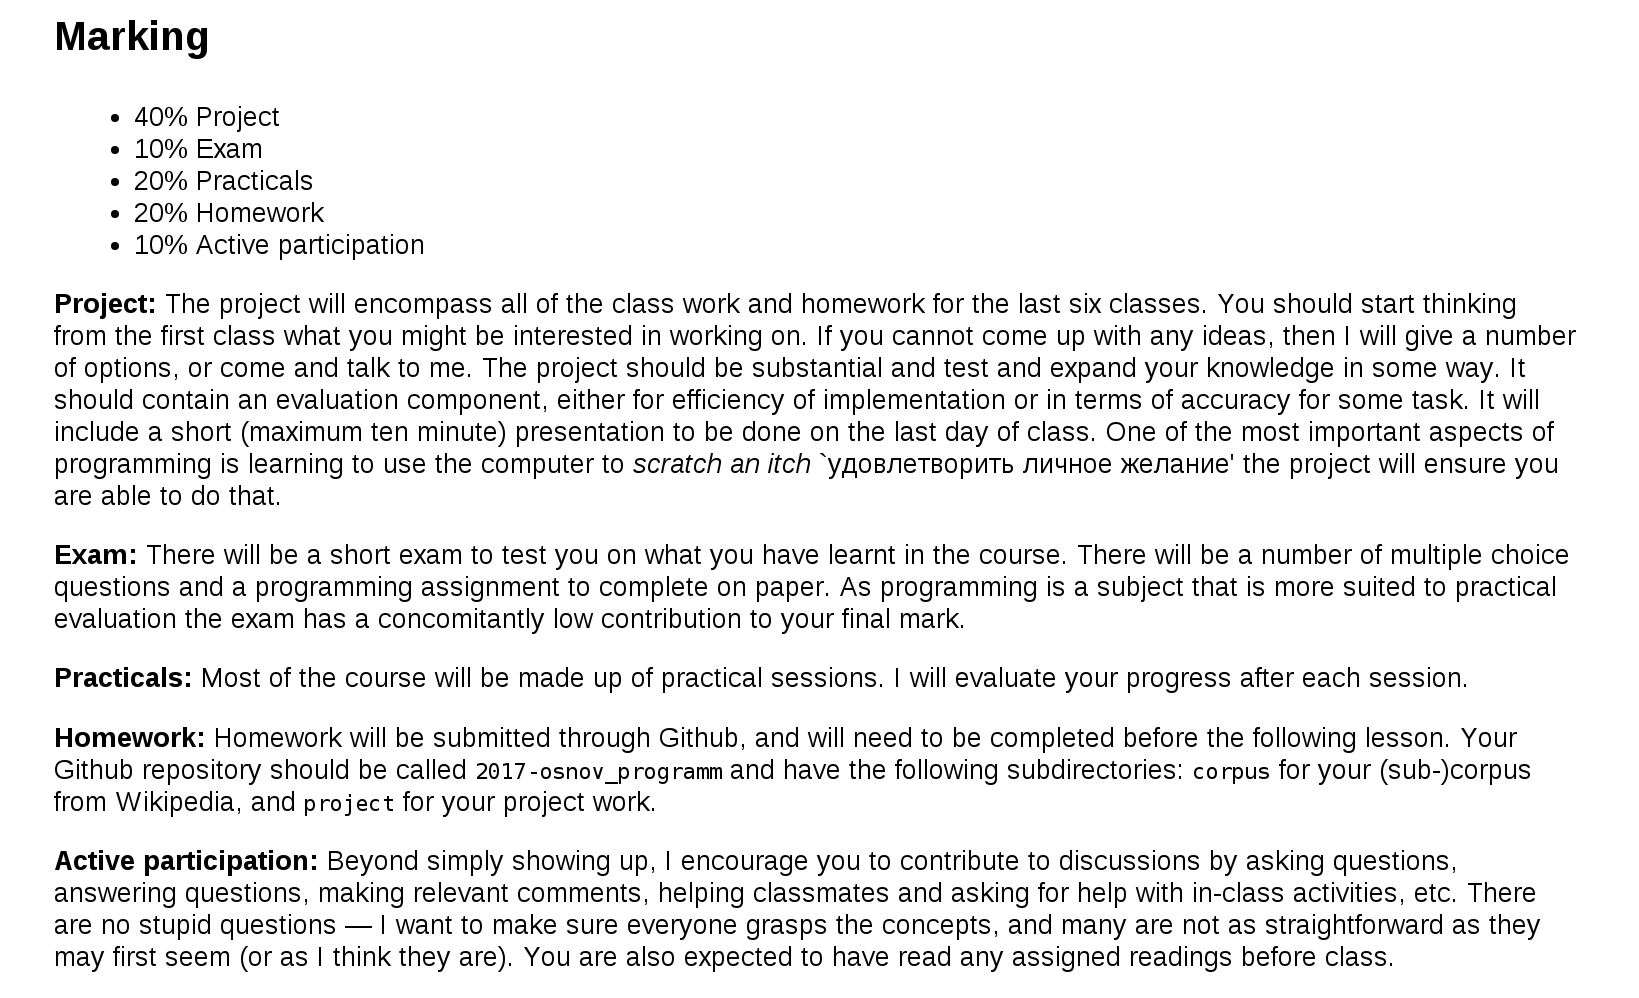
\includegraphics[width=0.8\textwidth]{graphics/course-page-marking.png}
\end{center}

\textbf{tl;dr} Most of the final mark is from the class work and project.

\end{frame}


\begin{frame}{What we are going to do today}

First things first:
\begin{itemize}
  \item Make sure you have Python installed
  \item Set up Github accounts
  \item Install a text editor
  \item Work with the shell
\end{itemize}

Then second things:
\begin{itemize}
  \item Choose a language 
  \begin{itemize}
    \item For purposes of speed, choose one with $<= 500,000$ articles
  \end{itemize}
  \item Download the Wikipedia in that language 
  \item Extract the text from Wikipedia
\end{itemize}



\end{frame}

\begin{frame}{Text editor}

% Sublime: +++
% TextWrangler: +
% Vim: +
% Atom: +
% Notepad++: +
% Emacs:


\end{frame}

\begin{frame}{Github}

All practical work will be stored and submitted through GitHub.

If you don't already have an account:
\begin{itemize}
 \item Go to \url{https://github.com/join}
 \item Fill in the information
 \item Click ``Create an account''
 \item Choose ``Unlimited public repositories for free.''
 \item Skip the next part.
\end{itemize}

\end{frame}

\begin{frame}[fragile]{Setup the directory structure}

In your browser:
\begin{itemize}
  \item First make a repository, call it {\tt 2017-osnov-programm}
  \item Choose `Initialise this repository with a README'
  \item Click `Clone or download' and copy the link
\end{itemize}

In the terminal:

\begin{verbatim}
$ git clone https://github.com/XXXXXX/2017-osnov-programm.git

$ cd 2017-osnov-programm

$ mkdir corpus project

\end{verbatim}

Where {\tt XXXXXX} is your GitHub username.



\end{frame}

\begin{frame}{Wikipedia as a corpus/1}

\begin{center}
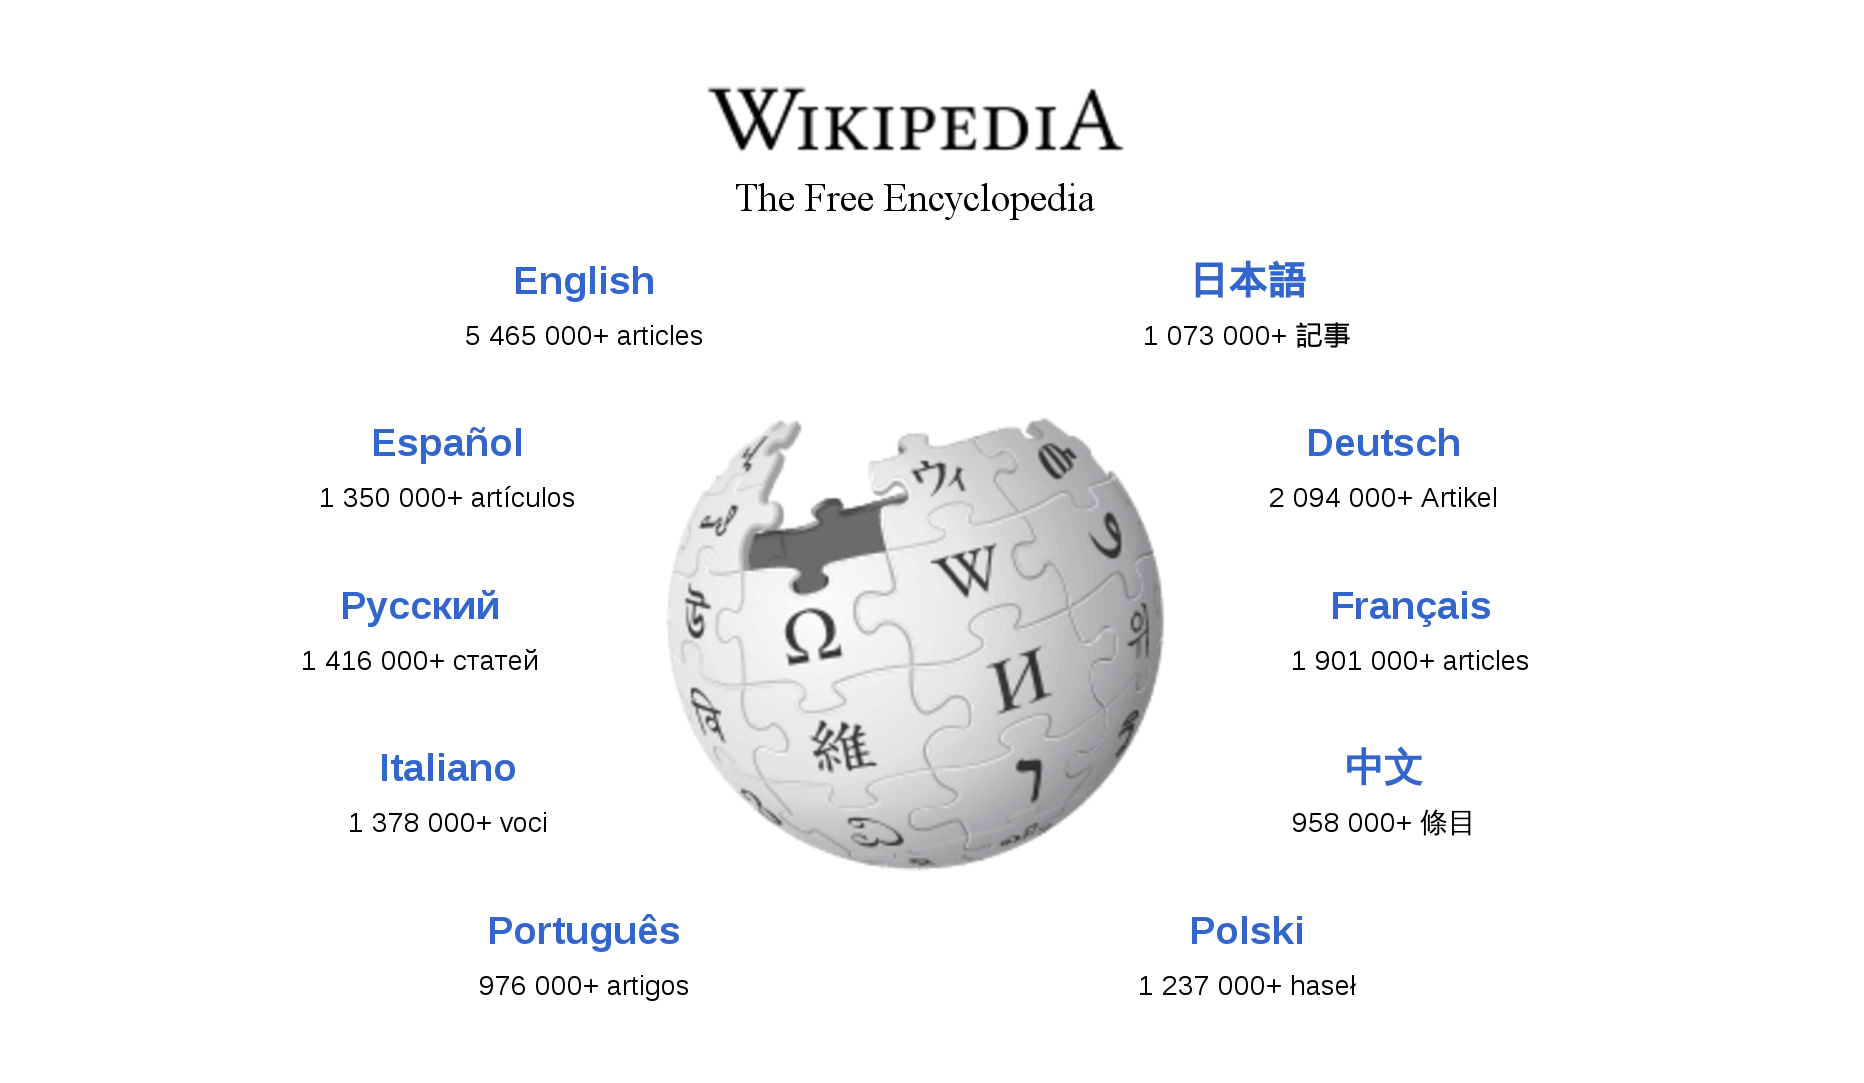
\includegraphics[width=0.70\textwidth]{graphics/wikipedia-front.png}
\end{center}

Wikipedia makes a great\footnote{Well, great in some respects} corpus:

\begin{itemize}
   \item Free to use and distribute
   \item Very many languages -- 295 at the last count
\end{itemize}

\end{frame}

\begin{frame}{Wikipedia as a corpus/2}

Deliberately vague steps:

\begin{itemize}
  \item Use your search engine to find where Wikipedia keeps it's `dumps'.
  \item Find the language code of the language you are interested in
  \item Download the dump for the language you are interested in
  \begin{itemize}
    \item Tip 1: You're looking for a `Database backup dump'
    \item Tip 2: The filename will include {\tt pages-articles.xml.bz2}
  \end{itemize}
  \item Find WikiExtractor on the Apertium Wiki
  \item Run WikiExtractor on the dump file you downloaded. 
\end{itemize}

\end{frame}

\begin{frame}[fragile]{What next}

There is an excellent introduction to the shell by Ken Church:


For the remainder of the class we'll be going through this and
making sure that you are able to run all of the commands.

Notes:
\begin{itemize}
  \item We'll use our Wikipedia dump, not Genesis
  \item Instead of {\tt tr -sc} we'll use {\tt tr -s} 
  \item Instead of {\tt [a-z][A-Z]} we'll use {\tt [,;:!?/." ()]} 
\end{itemize}

For example for Avar:
\begin{verbatim}
tr -s '[,;:!?/." ()]' '[\n*]' < wiki.txt | 
sort | grep '[а-яА-Я]' |
uniq -c > wiki.hist
\end{verbatim}

\end{frame}

\begin{frame}

You can get the same output in many different ways:

\begin{alltt}
\$ head -n 5 wiki.hist   \\
      2 100\% магӀарулал  \\
      1 10-го  \\
      1 11-абилеб  \\
      1 1250 км  \\
      1 1369-леб  \\
~  \\
\$ sed 5q wiki.hist   \\
      2 100\% магӀарулал  \\
      1 10-го  \\
      1 11-абилеб  \\
      1 1250 км  \\
      1 1369-леб  \\
~\\
\end{alltt}

\end{frame}



\end{document}

